\newpage
\section{Concept learning}
Il Concept Learning per esempio è la ricerca in spazi impotetici. Lo guardiamo perché è 
un'opportunità per dare uno sguardo ad un semplice apprendimento simbolico e come base per la sucessiva
introduzione di modelli flessibili.\\\\
Un altro caso sono gli spazi discreti (rappresentazione simbolica del bersaglio funzione), sono struttura dello
spazio delle ipotesi.\\\\
Il problema dell'apprendimento prevede di imparare come migliorare con l'esperienza in qualche compito. Migliorare oltre una task T,
tenendo conto di una misura di performance P e basandosi sull'esperienza E.

\begin{definition}
    Il concept learning si definisce come inferire una funzione booleana da esempi di tringing
    positivi e negativi.
    $$c: X \to \{t,f\} \:\:or\:\: \{+, -\} \:\:or\:\: \{yes, no\} \:\:or\:\: \{0,1\}$$
    con X che è lo spazio di instanze.
\end{definition}
\hspace{-15pt}Un esempio di concepts potrebberro essere "gatto" in animale o "sport-divertente" in giorni.
\begin{figure}[h!]
    \centering
    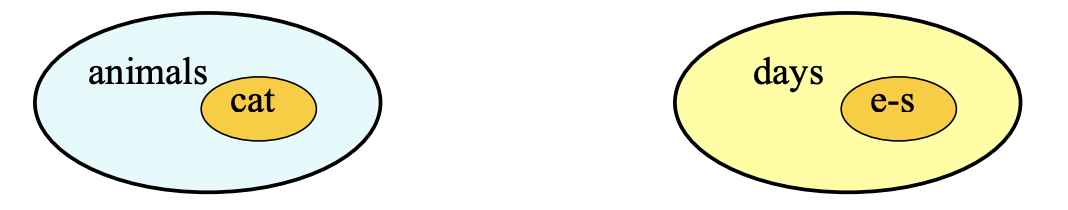
\includegraphics[width=0.5\textwidth]{images/ess-concept-learning.png}
\end{figure}
\begin{definition}
    Si definisce "\textbf{esempio}": $<x, c(x)>$ (o $<x,d>$) in D (o nell'insieme TR).
\end{definition}
\begin{definition}
    Si dice che $h: X\to \{0,1\}$ \textbf{soddisfa} $x$ se $h(x) = 1$
\end{definition}
\begin{definition}
    Una ipotesi $h$ è \textbf{consistente}
    \begin{itemize}
        \item Con un esempio $<x, c(x)>$, con $x \in X$ se $h(x) = c(x)$
        \item Con D, se $h(x) = c(x)$ per ogni esempio di training $<x, c(x)> \in D$
    \end{itemize}
\end{definition}
\begin{figure}[h!]
    \centering
    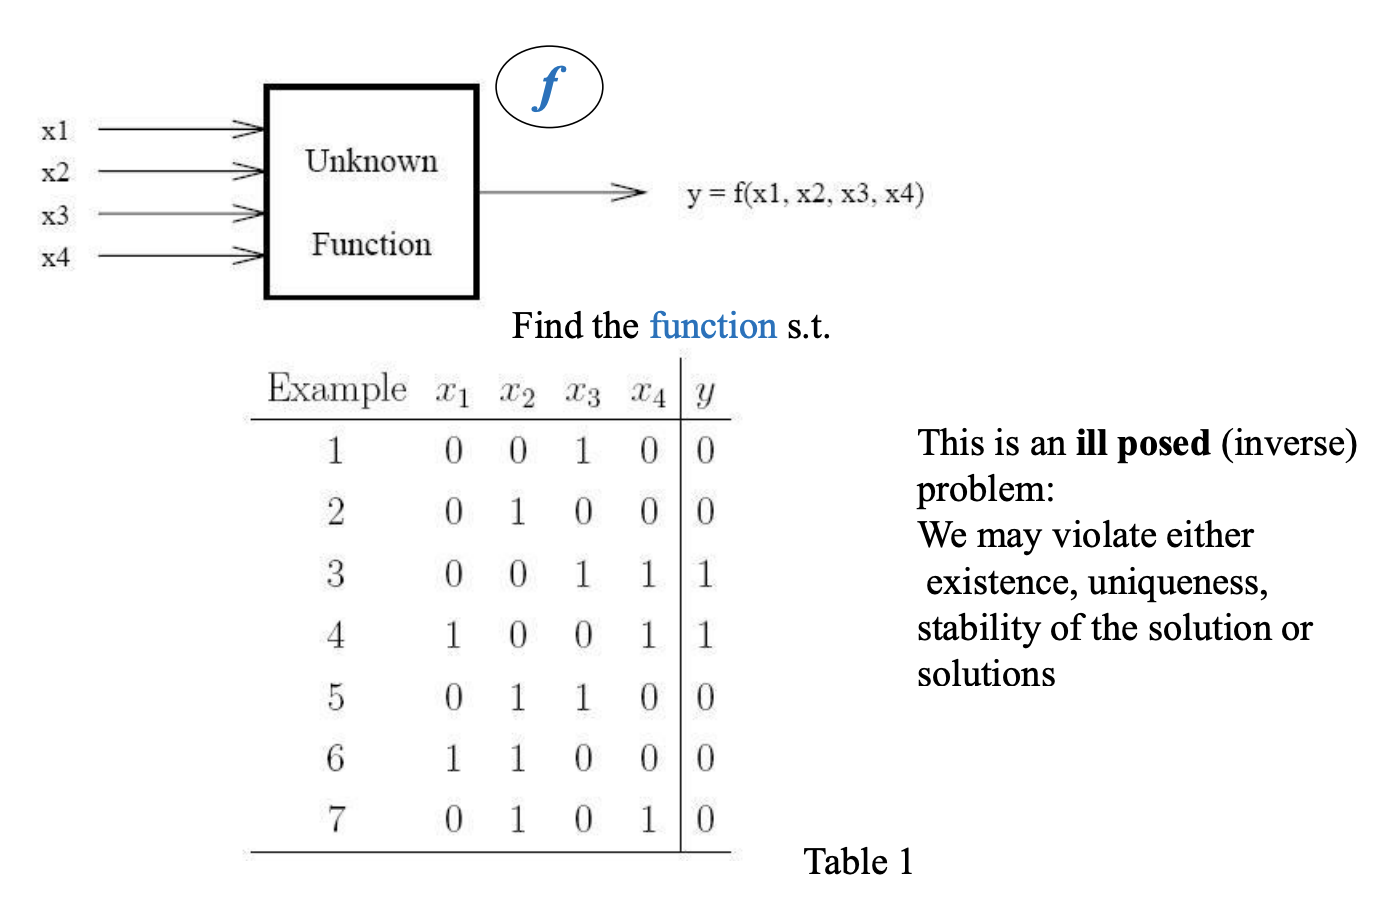
\includegraphics[width=0.65\textwidth]{images/learning-boolean-functions.png}
\end{figure}
\hspace{-15pt}Il problema dell'\textbf{ill posed} dice che: ci sono $2^{16} = 2^{2^4} = 65536$ possibili funzioni booleane
oltre quattro funzioni booleane di input. Noi non possiamo sapere quale sia corretta finché non abbiamo visto ogni possibile coppia
input-output. Dopo 7 esempi, noi continuiamo ad avere $2^9$ possibilità.
\begin{definition}
    Nel caso generale $|H| = 2^{\#-instances} = 2^{2^n}$ per inputs/outputs binari, e con n = dimensione input.
\end{definition}
\hspace{-15pt}\textbf{Per lavorare con spazi di ipotesi ristretti}: dobbiamo iniziare scegleindo uno spazio 
di ipotesi $H$ che è considerabile più piccolo rispetto allo spazio di tutte le possibili soluzioni.

\subsection{Regole congiuntive}
Quando ci chiediamo quante possibili $h$ abbiamo, è come chiedersi quante regole congiuntive semplici nell'esempio della tabella dei valori binari.\\
Nel caso generale:
\begin{itemize}
    \item Letterali positivi, per esempio: $h_1 = l_2 \:\:\: h_2 = (l_1 \land l_2) \:\:\: h_3 = true, \dots$\\
    \textbf{Regole congiuntive semplici} $|H| = 2^n$ (immaginando $l_i$ come un bit di una stringa di lunghezza n)
    \item Letterali (anche \textbf{not}($l_i$)) \hspace{15pt} $|H| = 3^n + 1$
\end{itemize}
\begin{example}
    Esempio di training per il concept.
    \begin{itemize}
        \item \textbf{Concept}: giorni il cui l'amico Aldo si diverte con il suo sport preferito.
        \item \textbf{Task}: prevedere il valore di "Enjoy Sport" per un giorno arbitrario in base ai valori degli altri attributi attributi.
    \end{itemize}
    \begin{figure}[h!]
        \centering
        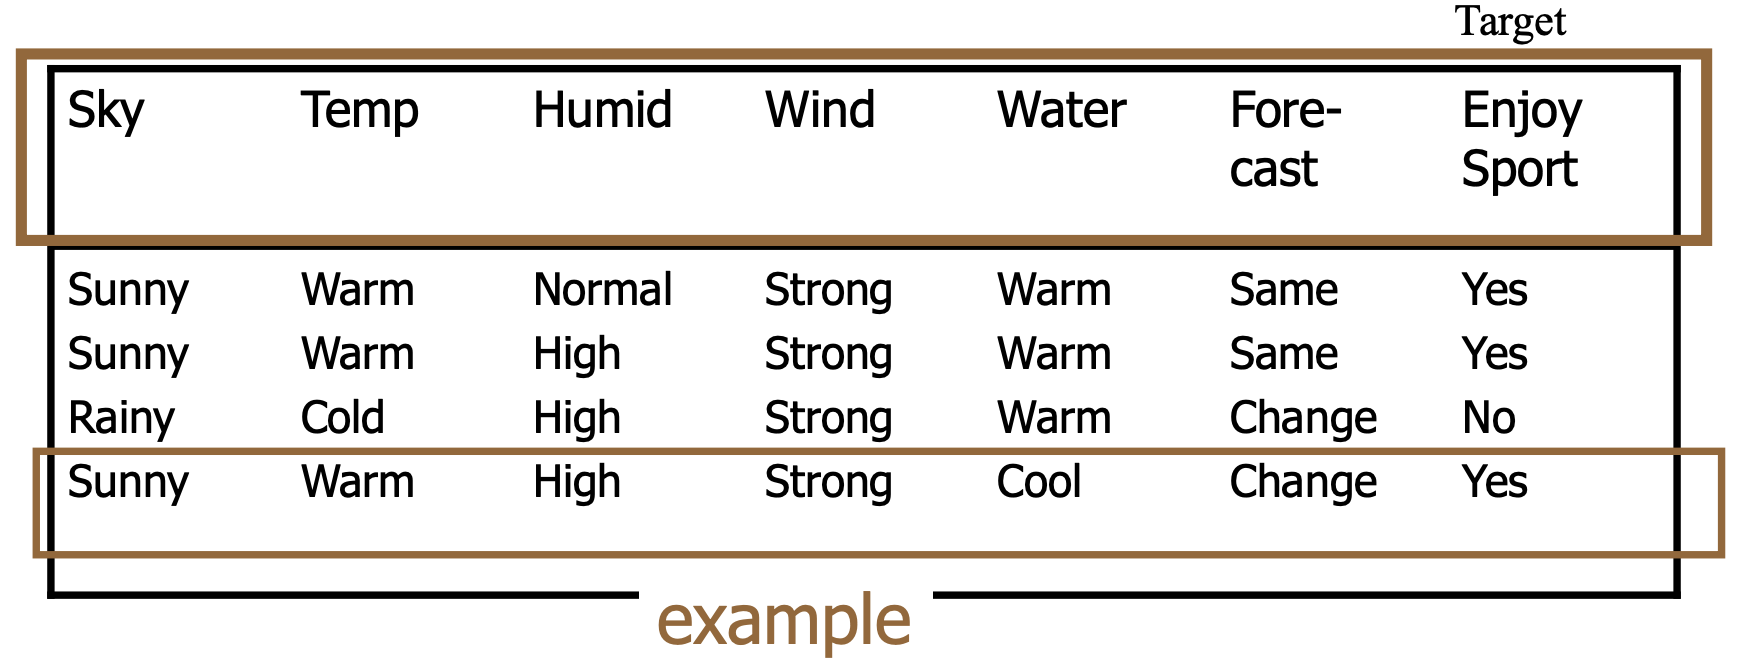
\includegraphics[width=0.5\textwidth]{images/training-esamples-concept-ler.png}
    \end{figure}
\end{example}
\subsubsection{Rappresentazione di ipotesi}
Un ipotesi $h$ è una congiunzione di vincoli sugli attributi. Ogni vincolo può contenere:
\begin{itemize}
    \item Uno specifico valore. Ess. Water=Warm
    \item Un valore che non mi interessa: Ess. Water=?
    \item Un valore non consetito (iporesi null). Ess. Water=$\O$
\end{itemize}
\begin{example}
    Un esempio di ipotesi $h$:\\
    Sky \hfill Temp \hfill Humid \hfill Wind \hfill Water \hfill Forecase\\
    Sunny \hfill ? \hfill ? \hfill Strong \hfill ? \hfill Same
    \begin{note}
        Questa è una funzione $h$, non un esempio di input.
    \end{note}
    \hspace{-15pt}Questa roba corrisponde alla funzione booleana:
    $$Sky = Sunny \land Wind = Strong \land Forecase = Same$$
    \begin{figure}[h!]
        \vspace{-15pt}
        \centering
        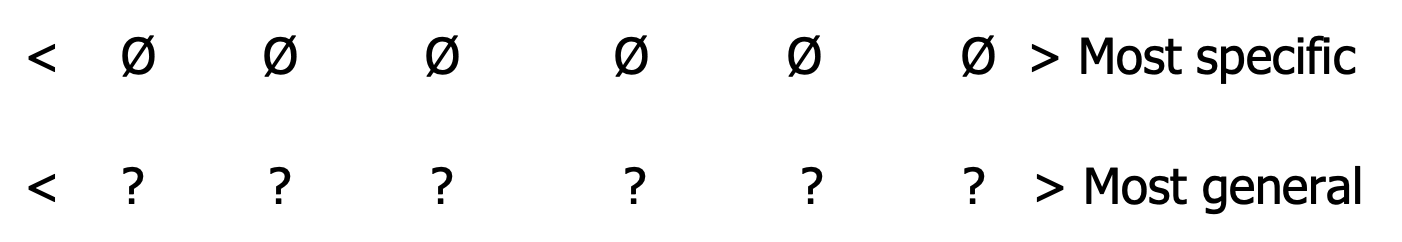
\includegraphics[width=0.5\textwidth]{images/rapre-ipotesi-ess.png}
    \end{figure}
\end{example}
\begin{definition}
    Task di apprendimento di concetti prototipici:
    \begin{itemize}
        \item \textbf{Given}
        \begin{itemize}
            \item \textbf{Istanza} X: Per esempio i possibili giorni descritti da degli attributi (Sky, Temp, Humidity, Wind, Water, Forecase)
            \item \textbf{Target function} c: EnjoySport X $\to \{0, 1\}$
            \item \textbf{Ipotesi H}: una congiunzione di (insieme finito di) letterali \\
            ess. $<$Sunny\:\: ? \:\:?\:\: Strong \:\:?\:\: Same $>$
            \item \textbf{Training examples} D: esempi positivi e negativi di una funzione target: $<x_1, c(x_1), \dots, <x_n, c(x_l)>$ ($l$ esempi)
        \end{itemize}
        \item \textbf{Trovare}: una ipotesi $h \in H$ tale che $h(x) = c(x)$ per ogni $x \in X$
    \end{itemize}
\end{definition}
Chiamiamo l'operazione di \textbf{Learning} la ricerca di ipotesi nello spazio $H$.\\\\
\textbf{Ipotesi dell'apprendimento induttivo}: Assumiamo in queste lezioni che "qualsiasi ipotesi trovata per approssimare la funzione target rispetto agli
esempi, andrà inoltre ad aprossimare la funzione target ben oltre gli esempi osservati".\\\\
$h=(x)$ per ogni $x \in D$ (ess. consistenza con D) \hspace{15pt} $h(x) = c(x)$ per ogni $x \in X$ \footnote{Un problema fondamentale del ML, analisi teorica ed empirica}\\\\
La rappresentazione per $H$ determina lo spazio di ricerca:
\begin{itemize}
    \item instance distinte: $3*2*2*2*2*2 = 96$
    \item Concetti distinti: $2^{96} = 2^{\#-instanze}$
    \item Ipotesi distinte sintatticamente (congiunzioni): $5*4*4*4*4*4 = 5120$ con 5 = sunny/cloudy/riny/?/$\O$ e 4=warm/cold/?/$\O$.
    \item Ipotesi distinte semanticamente: 1 + 4*3*3*3*3*3 = 973 (perché tutte le $h$ con $\O$ sono equivalenti a "false")
\end{itemize}
In generale: Dimensione elevata, addirittura infinita: strutturare lo spazio di ricerca può aiuto nella ricerca in modo più efficiente!

\subsubsection{Ordinamento da generale a specifico}
Consideriamo due ipotesi:
$$h_1 = <Sunny, ?, ?, Strong, ?, ?> \hspace{15pt} h_2 = <Sunny, ?, ?, ?, ?, ?>$$
Ed un insieme di instance coperte da $h_1$ e $h_2$.\\
$h_2$ impone meno vincoli rispetto a $h_1$ e quindi classifica più istanze x come positivo.
\begin{definition}
    Prendiamo $h_j$ e $h_k$ funzioni a valori booleani definite su X. Diciamo allora che $h_j$ è \textbf{più generale di o uguale a} $h_k$ (scritto come $h_j \geq h_k$) se e solo se
    $$\forall x \in X \: :\: [(h_k(x) = 1) \to (h_j(x) = 1)]$$
\end{definition}
\begin{example}
    Esempi binari $l_i: l_1 \geq (l_1 \land l_2),$ $l_1$ versus $l_2$, non comparabili. La relazione $\geq$ impone un 
    ordine di partizione (p.o.) sullo spazio di ipotesi $H$ che viene utilizzato da molti metodi di concept leargning. Possiamo approfittare di questo p.o. organizzare in modo efficiente la ricerca in H
\end{example}
